\documentclass[11pt, oneside]{article} 
\usepackage{geometry}
\geometry{letterpaper} 
\usepackage{graphicx}
	
\usepackage{amssymb}
\usepackage{amsmath}
\usepackage{parskip}
\usepackage{color}
\usepackage{hyperref}

\graphicspath{{/Users/telliott/Github/figures/}}
% \begin{center} \includegraphics [scale=0.4] {gauss3.png} \end{center}

\title{Pi is a constant}
\date{}

\begin{document}
\maketitle
\Large

%[my-super-duper-separator]

\label{sec:Pi_is_a_constant}

\begin{center}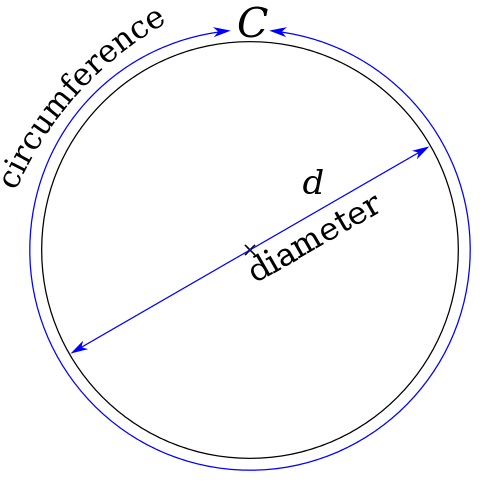
\includegraphics [scale=0.3] {circle0.png}\end{center}

We began the book with a bold claim:  the ratio of the circumference of a circle to its diameter is a constant, independent of the length of the diameter:
\[ \pi = \frac{C}{d} = \frac{C}{2r} \]

We did not prove this theorem at the time but will do so now.

We need the idea of limits, which was introduced previously, and a property of similar triangles.  The theorem is:  if two triangles are similar, then their sides are proportional to each other.

Consider an arc $a$ of a circle and two radii.  

The triangle corresponding to that arc has base $b$.  We can restate Archimedes argument about inscribed polygons by saying that, in the limit, as the inscribed polygon gets very close to being the same as the circle, $b \rightarrow a$.
\begin{center}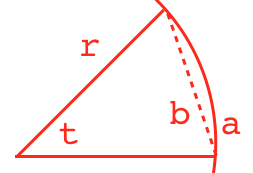
\includegraphics [scale=0.5] {similar3.png}\end{center}

So if there are $n$ pieces ($t = 2 \pi/n$), the ratio of the circumference to the arc is just $n$ and we have

\[ n = \frac{na}{a} = \frac{C}{a} = \frac{C}{b} \]
The last step is "in the limit."

Now draw a larger arc.  In the same way $b' \rightarrow a'$.
\begin{center}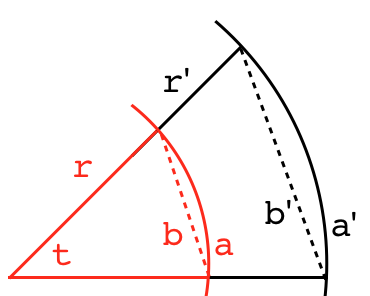
\includegraphics [scale=0.5] {similar4.png}\end{center}
and 
\[ n = \frac{C'}{b'} \]
since $t$ and $n$ haven't changed:
\[ n = \frac{C'}{b'} = \frac{C}{b} \]

But by similar triangles the ratios are equal:
\[ \frac{r}{b} = \frac{r'}{b'} \]
so
\[ \frac{C'}{C} = \frac{b'}{b} = \frac{r'}{r}\]
\[ \frac{C'}{r'} = \frac{C}{r}  \]

Suppose for a moment that $C = 2 \pi r$ and $C' = 2 \pi' r'$ and we don't know how $\pi$ compares to $\pi'$:

\[ \frac{2 \pi' r'}{r'} = \frac{2 \pi r}{r}  \]
We have that $\pi = \pi'$.

$\square$

Second proof:

Here is a simple variant which assumes something we will prove in the section on sine and cosine.  If this is confusing, it can easily be skipped.  

Drop the altitude $h$ in each of the two similar triangles.  The ratio $h/r$ is equal to $\sin t$, but the arc length is equal to $t$, measured in radians.

\begin{center}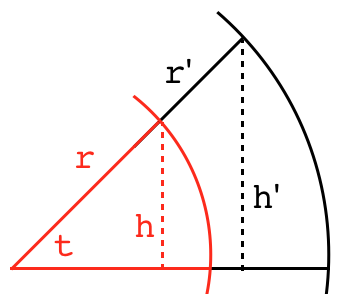
\includegraphics [scale=0.5] {similar5.png}\end{center}

In the limit that $n \rightarrow \infty$, the ratio between $t$ and $\sin t = h/r$ is equal to our "special limit":
\[ \lim_{n \rightarrow \infty} \ \frac{t}{\sin t} = 1 \]

If the ratio to the sine is equal to $1$, so is the ratio to its inverse and thus the ratio $s/r$ is constant, which is what we wanted to prove.

$\square$

\end{document}